% !TeX program = xelatex
\ifdefined\BookMaster\else
\documentclass[11pt,oneside]{article}
% !TeX program = xelatex
\usepackage[b5paper,left=22mm,right=22mm,top=20mm,bottom=22mm,footskip=11mm]{geometry}
\usepackage{fontspec}
\setmainfont{TeX Gyre Termes}
\setsansfont{TeX Gyre Heros}
\usepackage{amsmath,amssymb,mathtools,amsthm}
\renewcommand{\cdots}{\mathinner{\cdotp\cdotp\cdotp}}
\usepackage{graphicx,adjustbox,array,booktabs,longtable,multirow,enumitem,changepage,needspace}
\usepackage[table]{xcolor}
\usepackage{fancyhdr}
\raggedbottom
\interfootnotelinepenalty=10000
\newcommand{\BookFootnote}[2]{\begingroup\renewcommand{\thefootnote}{\fnsymbol{footnote}}\footnote[#1]{#2}\endgroup}
\newcommand{\BookFootnoteMark}[1]{\begingroup\renewcommand{\thefootnote}{\fnsymbol{footnote}}\footnotemark[#1]\endgroup}
\newcommand{\BookFootnoteText}[2]{\begingroup\renewcommand{\thefootnote}{\fnsymbol{footnote}}\footnotetext[#1]{#2}\endgroup}
\newenvironment{BookFloat}[1]{\par\addvspace{.6\baselineskip}\noindent\def\BookFloatID{#1}\begin{minipage}{\linewidth}\phantomsection\label{bookfloat:#1:start}}{\phantomsection\label{bookfloat:\BookFloatID:end}\end{minipage}\par\addvspace{.6\baselineskip}}

\usepackage[unicode,hidelinks]{hyperref}
\pagestyle{fancy}
\fancyhf{}
\newcommand{\BookFooter}{}
\fancyfoot[L]{\parbox[b]{\dimexpr\textwidth-15mm}{\footnotesize\BookFooter}}
\fancyfoot[R]{\footnotesize\thepage}
\renewcommand{\headrulewidth}{0pt}
\renewcommand{\footrulewidth}{0pt}
\setlength{\parindent}{0pt}
\setlength{\parskip}{0.2em}
\setlength{\emergencystretch}{3em}
\setlist{nosep,leftmargin=1.7em,labelsep=.65em}
\newif\ifBookNarrative
\BookNarrativetrue
\newenvironment{BookBody}{\setlength{\parindent}{0pt}}{}
\newcommand{\BookStatement}[1]{\par\addvspace{.6\baselineskip}\noindent #1\enspace\ignorespaces}
\newcommand{\BookLabel}[1]{\par\addvspace{.6\baselineskip}\needspace{3\baselineskip}\noindent\textbf{#1}\quad\ignorespaces}
\newcommand{\BookHeading}[1]{\par\addvspace{\baselineskip}\needspace{4\baselineskip}\noindent{\large\bfseries #1}\par\medskip}
\newcommand{\BookSubheading}[1]{\par\addvspace{.7\baselineskip}\needspace{3\baselineskip}\noindent{\bfseries #1}\par\smallskip}
\newcommand{\BookTextHeading}[1]{\par\addvspace{.7\baselineskip}\needspace{3\baselineskip}\noindent #1\par\smallskip}
\newcommand{\BookSectionTitle}[2]{\par\addvspace{1.2\baselineskip}\needspace{5\baselineskip}\noindent\colorbox{gray!25}{\sffamily\bfseries\small SECTION #1}\quad{\large\bfseries #2}\par\medskip}
\newcommand{\BookExerciseTitle}[1]{\par\addvspace{\baselineskip}\needspace{4\baselineskip}\noindent{\color{gray}\rule{1.5mm}{1.5mm}}\enspace{\large\bfseries Exercises #1}\par\medskip}
\newcommand{\BookBullet}[1]{\begin{list}{\textbullet}{\setlength{\leftmargin}{1.7em}\setlength{\labelwidth}{1em}\setlength{\labelsep}{.7em}\setlength{\topsep}{0pt}\setlength{\parsep}{0pt}\setlength{\itemsep}{0pt}}\item #1\end{list}}
\newcommand{\BookExercise}[2]{\begin{list}{\textbf{#1}}{\setlength{\leftmargin}{2.2em}\setlength{\labelwidth}{1.5em}\setlength{\labelsep}{.7em}\setlength{\topsep}{.15em}\setlength{\parsep}{0pt}\setlength{\itemsep}{0pt}}\item #2\end{list}}
\newcommand{\BookEnd}[1]{\unskip\nobreak\hfill\ensuremath{#1}}
\newcommand{\BookSource}[2]{\phantomsection\label{sourcepage:#1}} % Source-page anchors, retained through reflow.
\usepackage{multicol}
\usepackage{tikz}
\newcommand{\BookPartEntry}[2]{\par\noindent\makebox[17mm][l]{\bfseries Section #1}#2\par}
\newcommand{\BookPartTitle}[3]{\par\bigskip\noindent\begin{tikzpicture}\node[anchor=north west,inner sep=0pt,outer sep=0pt] (bookpart) at (0,0) {\begin{minipage}{\dimexpr\linewidth-.5pt}\hspace*{26mm}\begin{minipage}[t]{\dimexpr\linewidth-26mm}\begin{adjustbox}{max width=\linewidth}{\fontsize{20}{24}\selectfont\bfseries #2}\end{adjustbox}\par\vspace{6mm}\hrule\vspace{6mm}{\sffamily\footnotesize\setlength{\parskip}{.3em}#3}\vspace{3mm}\end{minipage}\end{minipage}};\path[shade,top color=gray!60,bottom color=white] (0,0) rectangle ([xshift=24mm]bookpart.south west);\node[anchor=north,font=\sffamily\bfseries\small] at (12mm,-2mm) {PART};\node[anchor=north,font=\sffamily\bfseries\Huge] at (12mm,-7mm) {#1};\end{tikzpicture}\par\bigskip}
\newsavebox{\BookMathBox}
\makeatletter
\newcommand{\BookInline}[1]{\leavevmode\hskip0pt\relax\begingroup\in@{\begin}{#1}\ifin@\sbox{\BookMathBox}{\(#1\)}\ifdim\wd\BookMathBox>\dimexpr\linewidth-1em\relax\resizebox{\dimexpr\linewidth-1em\relax}{!}{\usebox{\BookMathBox}}\else\(#1\)\fi\else\in@{\left}{#1}\ifin@\sbox{\BookMathBox}{\(#1\)}\ifdim\wd\BookMathBox>\dimexpr\linewidth-1em\relax\resizebox{\dimexpr\linewidth-1em\relax}{!}{\usebox{\BookMathBox}}\else\(#1\)\fi\else\(#1\)\fi\fi\endgroup\hskip0pt\relax}
\makeatother
\DeclareMathOperator{\Aut}{Aut}
\DeclareMathOperator{\End}{End}
\DeclareMathOperator{\Hom}{Hom}
\DeclareMathOperator{\GF}{GF}
\DeclareMathOperator{\irr}{irr}
\DeclareMathOperator{\lt}{lt}
\DeclareMathOperator{\lp}{lp}
\providecommand{\textcircled}[1]{\textnormal{(#1)}}

\begin{document}
\fi
\renewcommand{\BookFooter}{Section 27 Rings of Polynomials}
\pdfbookmark[0]{Section 27 Rings of Polynomials}{27_rings_of_polynomials}
\ifdefined\BookMaster\else\setcounter{page}{218}\fi
% Source PDF page 235; original printed page 218
\BookSource{235}{218}
\BookNarrativetrue

\begin{BookBody}

\BookSectionTitle{27}{Rings of Polynomials}

\BookTextHeading{\textbf{Polynomials in an Indeterminate}  }

\noindent We all have a pretty workable idea of what constitutes a\textit{ polynomial in} \BookInline{x} \textit{with coefficients} \textit{in} \BookInline{a} \textit{ring} \BookInline{R.} We can guess how to add and multiply such polynomials and know what is meant by the\textit{ degree} of a polynomial. We expect that the set \BookInline{R[x]} of all polynomials with coefficients in the ring \BookInline{R} is itself a ring with the usual operations of polynomial addition and multiplication, and that \BookInline{R} is a subring of \BookInline{R[x].} However, we will be working with polynomials from a slightly different viewpoint than the approach in high school algebra or calculus, and there are a few things that we want to say.

In the first place, we will call \BookInline{x} an\textbf{ indeterminate} rather than a variable. Suppose, for example that our ring of coefficients is \BookInline{\mathbb{Z}.} One of the polynomials in the ring \BookInline{\mathbb{Z}[x]} is \BookInline{1x,\allowbreak } which we shall write simply as \BookInline{x.} Now \BookInline{x} is not 1 or 2 or any of the other elements of \BookInline{\mathbb{Z}[x].} Thus from now on we will never write such things as “\BookInline{x= 1}” or “\BookInline{x= 2,\allowbreak }” as we have done in other courses. We call \BookInline{x} an indeterminate rather than a variable to emphasize this change. Also, we will never write an expression such as “\BookInline{x^{2}- 4= 0,\allowbreak }” simply because \BookInline{x^{2}- 4} is not the zero polynomial in our ring \BookInline{\mathbb{Z}[x].} We are accustomed to speaking of “solving a polynomial equation,” and will be spending a lot of time in the remainder of our text discussing this, but we will always refer to it as “finding a zero of a polynomial.” In summary, we try to be careful in our discussion of algebraic structures not to say in one context that things are equal and in another context that they are not equal.

If a person knows nothing about polynomials, it is not an easy task to describe precisely the nature of a polynomial in \BookInline{x} with coefficients in a ring \BookInline{R.} If we just define such a polynomial to be a\textit{ finite formal sum}

\begin{center}\begin{adjustbox}{max width=\linewidth}\BookInline{\displaystyle \sum _{i= 0}^{n}a_{i}x^{i}= a_{0}+ a_{1}x+ \cdots + a_{n}x^{n},\allowbreak }\end{adjustbox}\end{center}

\BookTextHeading{\ensuremath{\blacksquare} \textbf{HISTORICAL NOTE}  }

\noindent The use of \BookInline{x} and other letters near the end of the alphabet to represent an “indeterminate” is due to Rene´ Descartes (1596–1650). Earlier, Franc¸ois Viete (1540–1603) had used vowels for indeterminates and consonants for known quantities. Descartes is also responsible for the first publication of the factor theorem (Corollary 28.4) in his work\textit{ The Geometry,} which appeared as an appendix to his\textit{ Discourse on Method} (1637). This work also contained the first publication of the basic concepts of analytic geometry; Descartes showed how geometric curves can be described algebraically.

to reject as absolutely false everything of which he had the least doubt; but, since it was necessary that he who was thinking was “something,” he conceived his first principle of philosophy: “I think, therefore I am.” The most enlightening parts of the\textit{ Discourse on Method,} however, are the three appendices:\textit{ The Optics, The Geometry,} and\textit{ The Meteorology}. It was here that Descartes provided examples of how he actually applied his method. Among the important ideas Descartes discovered and published in these works were the sine law of refraction of light, the basics of the theory of equations, and a geometric explanation of the rainbow.

\noindent Descartes was born to a wealthy family in La Haye, France; since he was always of delicate health, he formed the habit of spending his mornings in bed. It was at these times that he accomplished his most productive work. The\textit{ Dis}\textit{course on Method} was Descartes’ attempt to show the proper procedures for “searching for truth in the sciences.” The first step in this process was

In 1649, Descartes was invited by Queen Christina of Sweden to come to Stockholm to tutor her. Unfortunately, the Queen required him, contrary to his long-established habits, to rise at an early hour. He soon contracted a lung disease and died in 1650.

\end{BookBody}

% Source PDF page 236; original printed page 219
\BookSource{236}{219}
\BookNarrativetrue

\begin{BookBody}

\noindent where \BookInline{a_{i}\in R,\allowbreak } we get ourselves into a bit of trouble. For surely \BookInline{0+ a_{1}x} and \BookInline{0+ a_{1}x+ } \BookInline{0x^{2}} are different as formal sums, but we want to regard them as the same polynomial. A practical solution to this problem is to define a polynomial as an\textit{ infinite formal sum}

\begin{center}\begin{adjustbox}{max width=\linewidth}\BookInline{\displaystyle \sum _{i= 0}^{\infty }a_{i}x^{i}= a_{0}+ a_{1}x+ \cdots + a_{n}x^{n}+ \cdots ,\allowbreak }\end{adjustbox}\end{center}

\noindent where \BookInline{a_{i}= 0} for all but a finite number of values of \BookInline{i.} Now there is no problem of having more than one finite formal sum represent what we wish to consider a single polynomial.

\BookLabel{27.1 Definition} Let \BookInline{R} be a ring. A\textbf{ polynomial} \BookInline{f(x)} \textbf{with coefficients in} \BookInline{R} is an infinite formal sum

\begin{center}\begin{adjustbox}{max width=\linewidth}\BookInline{\displaystyle \sum _{i= 0}^{\infty }a_{i}x^{i}= a_{0}+ a_{1}x+ \cdots + a_{n}x^{n}+ \cdots ,\allowbreak }\end{adjustbox}\end{center}

\noindent where \BookInline{a_{i}\in R} and for all but a finite number of values of \BookInline{i,\allowbreak a_{i}= 0.} The \BookInline{a_{i}} are\textbf{ coefficients} \textbf{of} \BookInline{f(x).} If for some \BookInline{i\geq 0} it is true that \BookInline{a_{i}\neq 0,\allowbreak } the largest such value of \BookInline{i} is the\textbf{ degree} \textbf{of} \BookInline{f(x).} If all \BookInline{a_{i}= 0,\allowbreak } then the degree of \BookInline{f(x)} is undefined.\label{bookfootnote:236:2:ref}\BookFootnote{2}{\label{bookfootnote:236:2:text}The degree of the zero polynomial is sometimes defined to be \BookInline{- 1,\allowbreak } which is the first integer less than 0, or defined to be \BookInline{- \infty } so that the degree of \BookInline{f(x)g(x)} will be the sum of the degrees of \BookInline{f(x)} and \BookInline{g(x)} if one of them is zero.} \BookEnd{\blacksquare}

To simplify working with polynomials, let us agree that if \BookInline{f(x)= a_{0}+ a_{1}x+ \cdots + } \BookInline{a_{n}x^{n}+ \cdots } has \BookInline{a_{i}= 0} for \BookInline{i>n,\allowbreak } then we may denote \BookInline{f(x)} by \BookInline{a_{0}+ a_{1}x+ \cdots + a_{n}x^{n}.} Also, if \BookInline{R} has unity \BookInline{1\neq 0,\allowbreak } we will write a term \BookInline{1x^{k}} in such a sum as \BookInline{x^{k}.} For example, in \BookInline{\mathbb{Z}[x],\allowbreak } we will write the polynomial \BookInline{2+ 1x} as \BookInline{2+ x.} Finally, we shall agree that we may omit altogether from the formal sum any term \BookInline{0x^{i},\allowbreak } or \BookInline{a_{0}} if \BookInline{a_{0}= 0} but not all \BookInline{a_{i}= 0.} Thus \BookInline{0,\allowbreak 2,\allowbreak x,\allowbreak } and \BookInline{2+ x^{2}} are polynomials with coefficients in \BookInline{\mathbb{Z}.} An element of \BookInline{R} is a \textbf{constant polynomial.}

Addition and multiplication of polynomials with coefficients in a ring \BookInline{R} are defined in a way familiar to us. If

\begin{center}\begin{adjustbox}{max width=\linewidth}\BookInline{\displaystyle f(x)= a_{0}+ a_{1}x+ \cdots + a_{n}x^{n}+ \cdots}\end{adjustbox}\end{center}

\noindent and

\begin{center}\begin{adjustbox}{max width=\linewidth}\BookInline{\displaystyle g(x)= b_{0}+ b_{1}x+ \cdots + b_{n}x^{n}+ \cdots ,\allowbreak }\end{adjustbox}\end{center}

\noindent then for polynomial addition, we have

\begin{center}\begin{adjustbox}{max width=\linewidth}\BookInline{\displaystyle f(x)+ g(x)= c_{0}+ c_{1}x+ \cdots + c_{n}x^{n}+ \cdots \;\text{where}\;c_{n}= a_{n}+ b_{n},\allowbreak }\end{adjustbox}\end{center}

\noindent and for polynomial multiplication, we have

\begin{center}\begin{adjustbox}{max width=\linewidth}\BookInline{\displaystyle f(x)g(x)= d_{0}+ d_{1}x+ \cdots + d_{n}x^{n}+ \cdots \;\text{where}\;d_{n}= \sum _{i= 0}^{n}a_{i}b_{n- i}}\end{adjustbox}\end{center}

\noindent Observe that both \BookInline{c_{i}} and \BookInline{d_{i}} are 0 for all but a finite number of values of \BookInline{i,\allowbreak } so these definitions make sense. Note that \BookInline{\sum _{i= 0}^{n}a_{i}b_{n- i}} need not equal \BookInline{\sum _{i= 0}^{n}b_{i}a_{n- i}} if \BookInline{R} is not commutative. With these definitions of addition and multiplication, we have the following theorem.

\BookLabel{27.2 Theorem} The set \BookInline{R[x]} of all polynomials in an indeterminate \BookInline{x} with coefficients in a ring \BookInline{R} is a ring under polynomial addition and multiplication. If \BookInline{R} is commutative, then so is \BookInline{R[x],\allowbreak } and if \BookInline{R} has unity \BookInline{1\neq 0,\allowbreak } then 1 is also unity for \BookInline{R[x].}

\BookLabel{\textit{Proof}} That \BookInline{\langle R[x],\allowbreak + \rangle } is an abelian group is apparent. The associative law for multiplication and the distributive laws are straightforward, but slightly cumbersome, computations. We illustrate by proving the associative law.

\end{BookBody}

% Source PDF page 237; original printed page 220
\BookSource{237}{220}
\BookNarrativetrue

\begin{BookBody}

Applying ring axioms to \BookInline{a_{i},\allowbreak b_{j},\allowbreak c_{k}\in R,\allowbreak } we obtain

\begin{center}\begin{adjustbox}{max width=\linewidth}\BookInline{\displaystyle \begin{aligned}\Bigg[\Bigg(\sum_{i=0}^{\infty} a_i x^i\Bigg)\Bigg(\sum_{j=0}^{\infty} b_j x^j\Bigg)\Bigg]\Bigg(\sum_{k=0}^{\infty} c_k x^k\Bigg)&= \Bigg[\sum_{n=0}^{\infty} \Bigg(\sum_{i=0}^{n} a_i b_{n-i}\Bigg)x^n\Bigg]\Bigg(\sum_{k=0}^{\infty} c_k x^k\Bigg)\\&= \sum_{s=0}^{\infty} \Bigg[\sum_{n=0}^{s} \Bigg(\sum_{i=0}^{n} a_i b_{n-i}\Bigg)c_{s-n}\Bigg]x^s\\&= \sum_{s=0}^{\infty} \Bigg(\sum_{i+j+k=s} a_i b_j c_k\Bigg)x^s\\&= \sum_{s=0}^{\infty} \Bigg[\sum_{m=0}^{s} a_{s-m}\Bigg(\sum_{j=0}^{m} b_j c_{m-j}\Bigg)\Bigg]x^s\\&= \Bigg(\sum_{i=0}^{\infty} a_i x^i\Bigg)\Bigg[\sum_{m=0}^{\infty} \Bigg(\sum_{j=0}^{m} b_j c_{m-j}\Bigg)x^m\Bigg]\\&= \Bigg(\sum_{i=0}^{\infty} a_i x^i\Bigg)\Bigg[\Bigg(\sum_{j=0}^{\infty} b_j x^j\Bigg)\Bigg(\sum_{k=0}^{\infty} c_k x^k\Bigg)\Bigg].\end{aligned}}\end{adjustbox}\end{center}

Whew! In this computation, the fourth expression, having just two summation signs, should be viewed as the value of the triple product \BookInline{f(x)g(x)h(x)} of these polynomials under this associative multiplication. (In a similar fashion, we view \BookInline{f(g(h(x)))} as the value of the associative composition \BookInline{(f\circ g\circ h)(x)} of three functions \BookInline{f,\allowbreak g,\allowbreak } and \BookInline{h.)}

The distributive laws are similarly proved. (See Exercise 26.)

The comments prior to the statement of the theorem show that \BookInline{R[x]} is a commutative ring if \BookInline{R} is commutative, and a unity \BookInline{1\neq 0} in \BookInline{R} is also unity for \BookInline{R[x],\allowbreak } in view of the definition of multiplication in \BookInline{R[x].}\BookEnd{\blacklozenge}

Thus \BookInline{\mathbb{Z}[x]} is the ring of polynomials in the indeterminate \BookInline{x} with integral coefficients\BookInline{,\allowbreak \mathbb{Q}[x]} the ring of polynomials in \BookInline{x} with rational coefficients, and so on.

\BookLabel{27.3 Example} In \BookInline{\mathbb{Z}_{2}[x],\allowbreak } we have

\begin{center}\begin{adjustbox}{max width=\linewidth}\BookInline{\displaystyle (x+ 1)^{2}= (x+ 1)(x+ 1)= x^{2}+ (1+ 1)x+ 1= x^{2}+ 1.}\end{adjustbox}\end{center}

\noindent Still working in \BookInline{\mathbb{Z}_{2}[x],\allowbreak } we obtain

\begin{center}\begin{adjustbox}{max width=\linewidth}\BookInline{\displaystyle (x+ 1)+ (x+ 1)= (1+ 1)x+ (1+ 1)= 0x+ 0= 0.}\end{adjustbox}\end{center} \BookEnd{\blacktriangle}

If \BookInline{R} is a ring and \BookInline{x} and \BookInline{y} are two indeterminates, then we can form the ring \BookInline{(R[x])[y],\allowbreak } that is, the ring of polynomials in \BookInline{y} with coefficients that are polynomials in \BookInline{x.} Every polynomial in \BookInline{y} with coefficients that are polynomials in \BookInline{x} can be rewritten in a natural way as a polynomial in \BookInline{x} with coefficients that are polynomials in \BookInline{y} as illustrated by Exercise 20. This indicates that \BookInline{(R[x])[y]} is naturally isomorphic to \BookInline{(R[y])[x],\allowbreak } although a careful proof is tedious. We shall identify these rings by means of this natural isomorphism, and shall consider this ring \BookInline{R[x,\allowbreak y]} the\textbf{ ring of polynomials in two inde}\textbf{terminates} \BookInline{x} \textbf{and} \BookInline{y} \textbf{with coefficients in} \BookInline{R.} The\textbf{ ring} \BookInline{R[x_{1},\allowbreak \cdots,\allowbreak x_{n}]} \textbf{of polynomials in} \textbf{the} \BookInline{n} \textbf{indeterminates} \BookInline{x_{i}} \textbf{with coefficients in} \BookInline{R} is similarly defined.

We leave as Exercise 24 the proof that if \BookInline{D} is an integral domain, then so is \BookInline{D[x].} In particular, if \BookInline{F} is a field, then \BookInline{F[x]} is an integral domain. Note that \BookInline{F[x]} is not a field, for \BookInline{x} is not a unit in \BookInline{F[x].} That is, there is no polynomial \BookInline{f(x)\in F[x]} such that \BookInline{xf(x)= 1.} By Theorem 26.6, one can construct the field of quotients \BookInline{F(x)} of \BookInline{F[x].} Any element in \BookInline{F(x)} can be represented as a quotient \BookInline{f(x)/g(x)} of two polynomials in \BookInline{F[x]} with

\end{BookBody}

% Source PDF page 238; original printed page 221
\BookSource{238}{221}
\BookNarrativetrue

\begin{BookBody}

\noindent \BookInline{g(x)\neq 0.} We similarly define \BookInline{F(x_{1},\allowbreak \cdots,\allowbreak x_{n})} to be the field of quotients of \BookInline{F[x_{1},\allowbreak \cdots,\allowbreak x_{n}].} This field \BookInline{F(x_{1},\allowbreak \cdots,\allowbreak x_{n})} is the\textbf{ field of rational functions in} \BookInline{n} \textbf{indeterminates over} \BookInline{F.} These fields play a very important role in algebraic geometry.

\BookTextHeading{\textbf{The Evaluation Homomorphisms}  }

\noindent We are now ready to proceed to show how homomorphisms can be used to study what we have always referred to as “solving a polynomial equation.” Let \BookInline{E} and \BookInline{F} be fields, with \BookInline{F} a subfield of \BookInline{E,\allowbreak } that is\BookInline{,\allowbreak F\leq E.} The next theorem asserts the existence of very important homomorphisms of \BookInline{F[x]} into \BookInline{E.} \textit{These homomorphisms will be the fundamental} \textit{tools for much of the rest of our work}.

\BookLabel{27.4 Theorem} \textbf{(The Evaluation Homomorphisms for Field Theory)} Let \BookInline{F} be a subfield of a field \BookInline{E,\allowbreak } let \BookInline{\alpha } be any element of \BookInline{E,\allowbreak } and let \BookInline{x} be an indeterminate. The map \BookInline{\phi _{\alpha }:F[x]\to E} defined by

\begin{center}\begin{adjustbox}{max width=\linewidth}\BookInline{\displaystyle \phi _{\alpha }\Big(a_{0}+ a_{1}x+ \cdots + a_{n}x^{n}\Big)= a_{0}+ a_{1}\alpha + \cdots + a_{n}\alpha ^{n}}\end{adjustbox}\end{center}

\noindent for \BookInline{(a_{0}+ a_{1}x+ \cdots + a_{n}x^{n})\in F[x]} is a homomorphism of \BookInline{F[x]} into \BookInline{E.} Also\BookInline{,\allowbreak \phi _{\alpha }(x)= \alpha,\allowbreak } and \BookInline{\phi _{\alpha }} maps \BookInline{F} isomorphically by the identity map; that is\BookInline{,\allowbreak \phi _{\alpha }(a)= a} for \BookInline{a\in F.} The homomorphism \BookInline{\phi _{\alpha }} is\textbf{ evaluation at} \BookInline{\alpha.}

\BookLabel{\textit{Proof}} The subfield and mapping diagram in Fig. 27.5 may help us to visualize this situation. The dashed lines indicate an element of the set. The theorem is really an immediate consequence of our definitions of addition and multiplication in \BookInline{F[x].} The map \BookInline{\phi _{\alpha }} is well defined, that is, independent of our representation of \BookInline{f(x)\in F[x]} as a finite sum

\begin{center}\begin{adjustbox}{max width=\linewidth}\BookInline{\displaystyle a_{0}+ a_{1}x+ \cdots + a_{n}x^{n},\allowbreak }\end{adjustbox}\end{center}

\noindent since such a finite sum representing \BookInline{f(x)} can be changed only by insertion or deletion of terms \BookInline{0x^{i},\allowbreak } which does not affect the value of \BookInline{\phi _{\alpha }(f(x)).}

If \BookInline{f(x)= a_{0}+ a_{1}x+ \cdots + a_{n}x^{n},\allowbreak g(x)= b_{0}+ b_{1}x+ \cdots + b_{m}x^{m},\allowbreak } and \BookInline{h(x)= f(x)+ } \BookInline{g(x)= c_{0}+ c_{1}x+ \cdots + c_{r}x^{r},\allowbreak } then

\begin{center}\begin{adjustbox}{max width=\linewidth}\BookInline{\displaystyle \phi _{\alpha }(f(x)+ g(x))= \phi _{\alpha }(h(x))= c_{0}+ c_{1}\alpha + \cdots + c_{r}\alpha ^{r},\allowbreak }\end{adjustbox}\end{center}

\noindent while

\begin{center}\begin{adjustbox}{max width=\linewidth}\BookInline{\displaystyle \phi _{\alpha }(f(x))+ \phi _{\alpha }(g(x))= \Big(a_{0}+ a_{1}\alpha + \cdots + a_{n}\alpha ^{n}\Big)+ \Big(b_{0}+ b_{1}\alpha + \cdots + b_{m}\alpha ^{m}\Big).}\end{adjustbox}\end{center}

\noindent Since by definition of polynomial addition we have \BookInline{c_{i}= a_{i}+ b_{i},\allowbreak } we see that

\begin{center}\begin{adjustbox}{max width=\linewidth}\BookInline{\displaystyle \phi _{\alpha }(f(x)+ g(x))= \phi _{\alpha }(f(x))+ \phi _{\alpha }(g(x)).}\end{adjustbox}\end{center}

\begin{BookFloat}{27_rings_of_polynomials-p238-15}
\begin{center}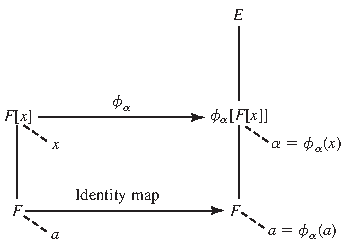
\includegraphics[width=0.473\linewidth,height=.8\textheight,keepaspectratio]{assets/p238_17.pdf}\end{center}
\begin{center}\small\textbf{27.5 Figure}\end{center}
\end{BookFloat}

\end{BookBody}

% Source PDF page 239; original printed page 222
\BookSource{239}{222}
\BookNarrativetrue

\begin{BookBody}

Turning to multiplication, we see that if

\begin{center}\begin{adjustbox}{max width=\linewidth}\BookInline{\displaystyle f(x)g(x)= d_{0}+ d_{1}x+ \cdots + d_{s}x^{s},\allowbreak }\end{adjustbox}\end{center}

\noindent then

\begin{center}\begin{adjustbox}{max width=\linewidth}\BookInline{\displaystyle \phi _{\alpha }(f(x)g(x))= d_{0}+ d_{1}\alpha + \cdots + d_{s}\alpha ^{s},\allowbreak }\end{adjustbox}\end{center}

\noindent while

\begin{center}\begin{adjustbox}{max width=\linewidth}\BookInline{\displaystyle [\phi _{\alpha }(f(x))][\phi _{\alpha }(g(x))]= \Big(a_{0}+ a_{1}\alpha + \cdots + \alpha _{n}\alpha ^{n}\Big)\Big(b_{0}+ b_{1}\alpha + \cdots + b_{m}\alpha ^{m}\Big).}\end{adjustbox}\end{center}

\noindent Since by definition of polynomial multiplication \BookInline{d_{j}= \sum _{i= 0}^{j}a_{i}b_{j- i},\allowbreak } we see that

\begin{center}\begin{adjustbox}{max width=\linewidth}\BookInline{\displaystyle \phi _{\alpha }(f(x)g(x))= [\phi _{\alpha }(f(x))][\phi _{\alpha }(g(x))].}\end{adjustbox}\end{center}

\noindent Thus \BookInline{\phi _{\alpha }} is a homomorphism.

The very definition of \BookInline{\phi _{\alpha }} applied to a constant polynomial \BookInline{a\in F[x],\allowbreak } where \BookInline{a\in F,\allowbreak } gives \BookInline{\phi _{\alpha }(a)= a,\allowbreak } so \BookInline{\phi _{\alpha }} maps \BookInline{F} isomorphically by the identity map. Again by definition of \BookInline{\phi _{\alpha },\allowbreak } we have \BookInline{\phi _{\alpha }(x)= \phi _{\alpha }(1x)= 1\alpha = \alpha.}\BookEnd{\blacklozenge}

We point out that this theorem is valid with the identical proof if \BookInline{F} and \BookInline{E} are merely commutative rings with unity rather than fields. However, we shall be interested primarily in the case in which they are fields.

It is hard to overemphasize the importance of this simple theorem for us. It is the very foundation for all of our further work in field theory. It is so simple that it could justifiably be called an\textit{ observation} rather than a theorem. It was perhaps a little misleading to write out the proof because the polynomial notation makes it look so complicated that you may be fooled into thinking it is a difficult theorem.

\BookLabel{27.6 Example} Let \BookInline{F} be \BookInline{\mathbb{Q}} and \BookInline{E} be \BookInline{\mathbb{R}} in Theorem 27.4, and consider the evaluation homomorphism \BookInline{\phi _{0}:\mathbb{Q}[x]\to \mathbb{R}.} Here

\begin{center}\begin{adjustbox}{max width=\linewidth}\BookInline{\displaystyle \phi _{0}\Big(a_{0}+ a_{1}x+ \cdots + a_{n}x^{n}\Big)= a_{0}+ a_{1}0+ \cdots + a_{n}0^{n}= a_{0}.}\end{adjustbox}\end{center}

\noindent Thus every polynomial is mapped onto its constant term. \BookEnd{\blacktriangle}

\BookLabel{27.7 Example} Let \BookInline{F} be \BookInline{\mathbb{Q}} and \BookInline{E} be \BookInline{\mathbb{R}} in Theorem 27.4 and consider the evaluation homomorphism \BookInline{\phi _{2}:\mathbb{Q}[x]\to \mathbb{R}.} Here

\begin{center}\begin{adjustbox}{max width=\linewidth}\BookInline{\displaystyle \phi _{2}\Big(a_{0}+ a_{1}x+ \cdots + a_{n}x^{n}\Big)= a_{0}+ a_{1}2+ \cdots + a_{n}2^{n}.}\end{adjustbox}\end{center}

\noindent Note that

\begin{center}\begin{adjustbox}{max width=\linewidth}\BookInline{\displaystyle \phi _{2}(x^{2}+ x- 6)= 2^{2}+ 2- 6= 0.}\end{adjustbox}\end{center}

\noindent Thus \BookInline{x^{2}+ x- 6} is in the kernel \BookInline{N} of \BookInline{\phi _{2}.} Of course,

\begin{center}\begin{adjustbox}{max width=\linewidth}\BookInline{\displaystyle x^{2}+ x- 6= (x- 2)(x+ 3),\allowbreak }\end{adjustbox}\end{center}

\noindent and the reason that \BookInline{\phi _{2}(x^{2}+ x- 6)= 0} is that \BookInline{\phi _{2}(x- 2)= 2- 2= 0.} \BookEnd{\blacktriangle}

\BookLabel{27.8 Example} Let \BookInline{F} be \BookInline{\mathbb{Q}} and \BookInline{E} be \BookInline{\mathbb{C}} in Theorem 27.4 and consider the evaluation homomorphism \BookInline{\phi _{i}:\mathbb{Q}[x]\to \mathbb{C}.} Here

\begin{center}\begin{adjustbox}{max width=\linewidth}\BookInline{\displaystyle \phi _{i}\Big(a_{0}+ a_{1}x+ \cdots + a_{n}x^{n}\Big)= a_{0}+ a_{1}i+ \cdots + a_{n}i^{n}}\end{adjustbox}\end{center}

\noindent and \BookInline{\phi _{i}(x)= i.} Note that

\begin{center}\begin{adjustbox}{max width=\linewidth}\BookInline{\displaystyle \phi _{i}(x^{2}+ 1)= i^{2}+ 1= 0,\allowbreak }\end{adjustbox}\end{center}

\noindent so \BookInline{x^{2}+ 1} is in the kernel \BookInline{N} of \BookInline{\phi _{i}.} \BookEnd{\blacktriangle}

\end{BookBody}

% Source PDF page 240; original printed page 223
\BookSource{240}{223}
\BookNarrativetrue

\begin{BookBody}

\BookLabel{27.9 Example} Let \BookInline{F} be \BookInline{\mathbb{Q}} and let \BookInline{E} be \BookInline{\mathbb{R}} in Theorem 27.4 and consider the evaluation homomorphism \BookInline{\phi _{\pi }:\mathbb{Q}[x]\to \mathbb{R}.} Here

\begin{center}\begin{adjustbox}{max width=\linewidth}\BookInline{\displaystyle \phi _{\pi }\Big(a_{0}+ a_{1}x+ \cdots + a_{n}x^{n}\Big)= a_{0}+ a_{1}\pi + \cdots + a_{n}\pi ^{n}.}\end{adjustbox}\end{center}

\noindent It can be proved that \BookInline{a_{0}+ a_{1}\pi + \cdots + a_{n}\pi ^{n}= 0} if and only if \BookInline{a_{i}= 0} for \BookInline{i= 0,\allowbreak 1,\allowbreak \cdots,\allowbreak n.} Thus the kernel of \BookInline{\phi _{\pi }} is \BookInline{\{0\},\allowbreak } and \BookInline{\phi _{\pi }} is a one-to-one map. This shows that all\textit{ formal} \textit{polynomials in} \BookInline{\pi } \textit{with rational coefficients} form a ring isomorphic to \BookInline{\mathbb{Q}[x]} in a natural way with \BookInline{\phi _{\pi }(x)= \pi.}\BookEnd{\blacktriangle}

\BookTextHeading{\textbf{The New Approach}  }

\noindent We now complete the connection between our new ideas and the classical concept of solving a polynomial equation. Rather than speak of\textit{ solving} \BookInline{a} \textit{polynomial equation,} we shall refer to\textit{ finding} \BookInline{a} \textit{zero of} \BookInline{a} \textit{polynomial}.

\BookLabel{27.10 Definition} Let \BookInline{F} be a subfield of a field \BookInline{E,\allowbreak } and let \BookInline{\alpha } be an element of \BookInline{E.} Let \BookInline{f(x)= a_{0}+ } \BookInline{a_{1}x+ \cdots + a_{n}x^{n}} be in \BookInline{F[x],\allowbreak } and let \BookInline{\phi _{\alpha }:F[x]\to E} be the evaluation homomorphism of Theorem 27.4. Let \BookInline{f(\alpha )} denote

\begin{center}\begin{adjustbox}{max width=\linewidth}\BookInline{\displaystyle \phi _{\alpha }(f(x))= a_{0}+ a_{1}\alpha + \cdots + a_{n}\alpha ^{n}.}\end{adjustbox}\end{center}

\noindent If \BookInline{f(\alpha )= 0,\allowbreak } then \BookInline{\alpha } is a\textbf{ zero of} \BookInline{f(x).} \BookEnd{\blacksquare}

In terms of this definition, we can rephrase the classical problem of finding all real numbers \BookInline{r} such that \BookInline{r^{2}+ r- 6= 0} by letting \BookInline{F= \mathbb{Q}} and \BookInline{E= \mathbb{R}} and\textit{ finding all} \BookInline{\alpha \in \mathbb{R}} \textit{such that}

\begin{center}\begin{adjustbox}{max width=\linewidth}\BookInline{\displaystyle \phi _{\alpha }(x^{2}+ x- 6)= 0,\allowbreak }\end{adjustbox}\end{center}

\noindent \textit{that is, finding all zeros of} \BookInline{x^{2}+ x- 6} in \BookInline{\mathbb{R}.} Both problems have the same answer, since

\begin{center}\begin{adjustbox}{max width=\linewidth}\BookInline{\displaystyle \{\alpha \in \mathbb{R}\mid \phi _{\alpha }(x^{2}+ x- 6)= 0\}= \{r\in \mathbb{R}\mid r^{2}+ r- 6= 0\}= \{2,\allowbreak - 3\}.}\end{adjustbox}\end{center}

It may seem that we have merely succeeded in making a simple problem seem quite complicated. In fact,\textit{ what we have done is to phrase the problem in the language} \textit{of mappings, and we can now use all the mapping machinery that we have developed} \textit{and will continue to develop for its solution}.

\BookTextHeading{\textbf{Our Basic Goal}  }

\noindent We continue to attempt to put our future work in perspective. Sections 30 and 31 are concerned with topics in ring theory that are analogous to the material on factor groups and homomorphisms for group theory. However, our aim in developing these analogous concepts for rings will be quite different from our aims in group theory. In group theory we used the concepts of factor groups and homomorphisms to study the structure of a given group and to determine the types of group structures of certain orders that could exist. We will be talking about homomorphisms and factor rings in Section 30 with an eye to finding zeros of polynomials, which is one of the oldest and most fundamental problems in algebra. Let us take a moment to talk about this aim in the light of mathematical history, using the language of “solving polynomial equations” to which we are accustomed.

We start with the Pythagorean school of mathematics of about 525 B.C. The Pythagoreans worked with the assumption that all distances are\textbf{ commensurable}; that is, given distances \BookInline{a} and \BookInline{b,\allowbreak } there should exist a unit of distance \BookInline{u} and integers \BookInline{n} and \BookInline{m} such that \BookInline{a= (n)(u)} and \BookInline{b= (m)(u).} In terms of numbers, then, thinking of \BookInline{u} as being 
% Source PDF page 241; original printed page 224
\BookSource{241}{224}
one unit of distance, they maintained that all numbers are integers. This idea of commensurability can be rephrased according to our ideas as an assertion that all numbers are rational, for if \BookInline{a} and \BookInline{b} are rational numbers, then each is an integral multiple of the reciprocal of the least common multiple of their denominators. For example, if \BookInline{a= \frac{7}{12}} and \BookInline{b= \frac{19}{15},\allowbreak } then \BookInline{a= (35)(\frac{1}{60})} and \BookInline{b= (76)(\frac{1}{60}).}

\end{BookBody}

\BookNarrativetrue

\begin{BookBody}

The Pythagoreans knew, of course, what is now called the\textit{ Pythagorean theorem;} that is, for a right triangle with legs of lengths \BookInline{a} and \BookInline{b} and a hypotenuse of length \BookInline{c,\allowbreak }

\begin{center}\begin{adjustbox}{max width=\linewidth}\BookInline{\displaystyle a^{2}+ b^{2}= c^{2}.}\end{adjustbox}\end{center}

\noindent They also had to grant the existence of a hypotenuse of a right triangle having two legs of equal length, say one unit each. The hypotenuse of such a right triangle would, as we know, have to have a length of \BookInline{\sqrt{2}.} Imagine then their consternation and dismay when one of their society—according to some stories it was Pythagoras himself— came up with the embarrassing fact that is stated in our terminology in the following theorem.

\BookLabel{27.11 Theorem} The polynomial \BookInline{x^{2}- 2} has no zeros in the rational numbers. Thus \BookInline{\sqrt{2}} is not a rational number.

\BookLabel{\textit{Proof}} Suppose that \BookInline{m/n} for \BookInline{m,\allowbreak n\in \mathbb{Z}} is a rational number such that \BookInline{(m/n)^{2}= 2.} We assume that we have canceled any factors common to \BookInline{m} and \BookInline{n,\allowbreak } so that the fraction \BookInline{m/n} is in lowest terms with gcd\BookInline{(m,\allowbreak n)= 1.} Then

\begin{center}\begin{adjustbox}{max width=\linewidth}\BookInline{\displaystyle m^{2}= 2n^{2},\allowbreak }\end{adjustbox}\end{center}

\noindent where both \BookInline{m^{2}} and \BookInline{2n^{2}} are integers. Since \BookInline{m^{2}} and \BookInline{2n^{2}} are the same integer, and since 2 is a factor of \BookInline{2n^{2},\allowbreak } we see that 2 must be one of the factors of \BookInline{m^{2}.} But as a square, \BookInline{m^{2}} has as factors the factors of \BookInline{m} repeated twice. Thus \BookInline{m^{2}} must have two factors 2. Then \BookInline{2n^{2}} must have two factors 2, so \BookInline{n^{2}} must have 2 as a factor, and consequently \BookInline{n} has 2 as a factor. We have deduced from \BookInline{m^{2}= 2n^{2}} that both \BookInline{m} and \BookInline{n} must be divisible by 2, contradicting the fact that the fraction \BookInline{m/n} is in lowest terms. Thus we have \BookInline{2\neq (m/n)^{2}} for any \BookInline{m,\allowbreak n\in \mathbb{Z}.}\BookEnd{\blacklozenge}

\BookTextHeading{\ensuremath{\blacksquare} \textbf{HISTORICAL NOTE}  }

\noindent The solution of polynomial equations has been a goal of mathematics for nearly 4000 years. The Babylonians developed versions of the quadratic formula to solve quadratic equations. For example, to solve \BookInline{x^{2}- x= 870,\allowbreak } the Babylonian scribe instructed his students to take half of 1 ( 21 ), square it ( 41 ), and add that to 870. The square root of 870 14, namely 29 12, is then added to \BookInline{\frac{1}{2}} to give 30 as the answer. What the scribes did not discuss, however, was what to do if the square root in this process was not a rational number. Chinese mathematicians, however, from about 200 B.C., discovered a method similar to what is now called\textit{ Horner’}\BookInline{s} \textit{method} to solve quadratic equations numerically; since they used a decimal system, they were able in principle to carry out the computation to as many places as necessary and could therefore ignore the distinction between rational and irrational solutions. The Chinese, in fact, extended their numerical techniques to polynomial equations of higher degree. In the Arab world, the Persian poet–mathematician Omar Khayyam (1048–1131) developed methods for solving cubic equations geometrically by finding the point(s) of intersection of appropriately chosen conic sections, while Sharaf al-Din al-Tusi (died 1213) used, in effect, techniques of calculus to determine whether or not a cubic equation had a real positive root. It was the Italian Girolamo Cardano (1501–1576) who first published a procedure for solving cubic equations algebraically.

\end{BookBody}

% Source PDF page 242; original printed page 225
\BookSource{242}{225}
\BookNarrativetrue

\begin{BookBody}

\textit{Thus the Pythagoreans} \BookInline{ran} \textit{right into the question of} \BookInline{a} \textit{solution of} \BookInline{a} \textit{polynomial} \textit{equation}\BookInline{,\allowbreak x^{2}- 2= 0.} We refer the student to Shanks [36, Chapter 3], for a lively and totally delightful account of this Pythagorean dilemma and its significance in mathematics.

In our motivation of the definition of a group, we commented on the necessity of having negative numbers, so that equations such as \BookInline{x+ 2= 0} might have solutions. The introduction of negative numbers caused a certain amount of consternation in some philosophical circles. We can visualize 1 apple, 2 apples, and even \BookInline{\frac{13}{11}} apples, but how can we point to anything and say that it is \BookInline{- 17} apples? Finally, consideration of the equation \BookInline{x^{2}+ 1= 0} led to the introduction of the number \BookInline{i.} The very name of an “imaginary number” given to \BookInline{i} shows how this number was regarded. Even today, many students are led by this name to regard \BookInline{i} with some degree of suspicion. The negative numbers were introduced to us at such an early stage in our mathematical development that we accepted them without question.

We first met polynomials in high school freshman algebra. The first problem there was to learn how to add, multiply, and factor polynomials. Then, in both freshman algebra and in the second course in algebra in high school, considerable emphasis was placed on solving polynomial equations. These topics are exactly those with which we shall be concerned. The difference is that while in high school, only polynomials with real number coefficients were considered,\textit{ we shall be doing our work for polynomials} \textit{with coefficients from any} \BookInline{\text{fi}eld.}

Once we have developed the machinery of homomorphisms and factor rings in Section 30, we will proceed with our\textbf{ basic goal}: to show that given any polynomial of degree \BookInline{\geq 1,\allowbreak } where the coefficients of the polynomial may be from any field, we can find a zero of this polynomial in some field containing the given field. After the machinery is developed in Sections 30 and 31, the achievement of this goal will be very easy, and is really a very elegant piece of mathematics.

All this fuss may seem ridiculous, but just think back in history. This is the\textit{ culmi}\textit{nation of more than 2000 years of mathematical endeavor in working with polynomial} \textit{equations}. After achieving our\textit{ basic goal,} we shall spend the rest of our time studying the nature of these solutions of polynomial equations. We need have no fear in approaching this material.\textit{ We shall be dealing with familiar topics of high school algebra. This} \textit{work should seem much more natural than group theory}.

In conclusion, we remark that the machinery of factor rings and ring homomorphisms is not really necessary in order for us to achieve our\textit{ basic goal}. For a direct demonstration, see Artin [27, p. 29]. However, factor rings and ring homomorphisms are fundamental ideas that we should grasp, and our\textit{ basic goal} will follow very easily once we have mastered them.

\end{BookBody}

\BookNarrativefalse

\begin{BookBody}

\BookExerciseTitle{27}

\BookTextHeading{\textbf{Computations}}

\noindent In Exercises 1 through 4, find the sum and the product of the given polynomials in the given polynomial ring.

\BookExercise{1.}{\BookInline{f(x)= 4x- 5,\allowbreak g(x)= 2x^{2}- 4x+ 2} in \BookInline{\mathbb{Z}_{8}[x].}}

\BookExercise{2.}{\BookInline{f(x)= x+ 1,\allowbreak g(x)= x+ 1} in \BookInline{\mathbb{Z}_{2}[x].}}

\BookExercise{3.}{\BookInline{f(x)= 2x^{2}+ 3x+ 4,\allowbreak g(x)= 3x^{2}+ 2x+ 3} in \BookInline{\mathbb{Z}_{6}[x].}}

\BookExercise{4.}{\BookInline{f(x)= 2x^{3}+ 4x^{2}+ 3x+ 2,\allowbreak g(x)= 3x^{4}+ 2x+ 4} in \BookInline{\mathbb{Z}_{5}[x].}}

\BookExercise{5.}{How many polynomials are there of degree \BookInline{\leq 3} in \BookInline{\mathbb{Z}_{2}[x]}? (Include 0.)}

\BookExercise{6.}{How many polynomials are there of degree \BookInline{\leq 2} in \BookInline{\mathbb{Z}_{5}[x]}? (Include 0.)}

\end{BookBody}

% Source PDF page 243; original printed page 226
\BookSource{243}{226}
\BookNarrativefalse

\begin{BookBody}

\noindent In Exercises 7 and \BookInline{8,\allowbreak F= E= \mathbb{C}} in Theorem 27.4. Compute for the indicated evaluation homomorphism.

\BookExercise{7.}{\BookInline{\phi _{2}(x^{2}+ 3)}}

\BookExercise{8.}{\BookInline{\phi _{i}(2x^{3}- x^{2}+ 3x+ 2)}}

\noindent In Exercises 9 through \BookInline{11,\allowbreak F= E= \mathbb{Z}_{7}} in Theorem 27.4. Compute for the indicated evaluation homomorphism.

\BookExercise{9.}{\BookInline{\phi _{3}[(x^{4}+ 2x)(x^{3}- 3x^{2}+ 3)]}}

\BookExercise{10.}{\BookInline{\phi _{5}[(x^{3}+ 2)(4x^{2}+ 3)(x^{7}+ 3x^{2}+ 1)]}}

\BookExercise{11.}{\BookInline{\phi _{4}(3x^{106}+ 5x^{99}+ 2x^{53})[}\textit{Hint:} Use Fermat’s theorem.]}

\noindent In Exercises 12 through 15, find all zeros in the indicated finite field of the given polynomial with coefficients in that field. [\textit{Hint:} One way is simply to try all candidates!]

\BookExercise{12.}{\BookInline{x^{2}+ 1} in \BookInline{\mathbb{Z}_{2}}}

\BookExercise{13.}{\BookInline{x^{3}+ 2x+ 2} in \BookInline{\mathbb{Z}_{7}}}

\BookExercise{14.}{\BookInline{x^{5}+ 3x^{3}+ x^{2}+ 2x} in \BookInline{\mathbb{Z}_{5}}}

\BookExercise{15.}{\BookInline{f(x)g(x)} where \BookInline{f(x)= x^{3}+ 2x^{2}+ 5} and \BookInline{g(x)= 3x^{2}+ 2x} in \BookInline{\mathbb{Z}_{7}}}

\BookExercise{16.}{Let \BookInline{\phi _{a}:\mathbb{Z}_{5}[x]\to \mathbb{Z}_{5}} be an evaluation homomorphism as in Theorem 27.4. Use Fermat’s theorem to evaluate \BookInline{\phi _{3}(x^{231}+ 3x^{117}- 2x^{53}+ 1).}}

\BookExercise{17.}{Use Fermat’s theorem to find all zeros in \BookInline{\mathbb{Z}_{5}} of \BookInline{2x^{219}+ 3x^{74}+ 2x^{57}+ 3x^{44}.}}

\BookTextHeading{\textbf{Concepts}}

\noindent In Exercises 18 and 19, correct the definition of the italicized term without reference to the text, if correction is needed, so that it is in a form acceptable for publication.

\BookExercise{18.}{A\textit{ polynomial with coefficients in} \BookInline{a} \textit{ring} \BookInline{R} \textit{is an infinite formal sum}}

\begin{center}\begin{adjustbox}{max width=\linewidth}\BookInline{\displaystyle \sum _{i= 0}^{\infty }a_{i}x^{i}= a_{0}+ a_{1}x+ a_{2}x^{2}+ \cdots + a_{n}x^{n}+ \cdots}\end{adjustbox}\end{center}

where \BookInline{a_{i}\in R} for \BookInline{i= 0,\allowbreak 1,\allowbreak 2,\allowbreak \cdots.}

\BookExercise{19.}{Let \BookInline{F} be a field and let \BookInline{f(x)\in F[x].} A\textit{ zero of} \BookInline{f(x)} is an \BookInline{\alpha \in F} such that \BookInline{\phi _{\alpha }(f(x))= 0,\allowbreak } where \BookInline{\phi _{\alpha }:F(x)\to F} is the evaluation homomorphism mapping \BookInline{x} into \BookInline{\alpha.}}

\BookExercise{20.}{Consider the element}

\begin{center}\begin{adjustbox}{max width=\linewidth}\BookInline{\displaystyle f(x,\allowbreak y)= (3x^{3}+ 2x)y^{3}+ (x^{2}- 6x+ 1)y^{2}+ (x^{4}- 2x)y+ (x^{4}- 3x^{2}+ 2)}\end{adjustbox}\end{center}

of \BookInline{(\mathbb{Q}[x])[y].} Write \BookInline{f(x,\allowbreak y)} as it would appear if viewed as an element of \BookInline{(\mathbb{Q}[y])[x].}

\BookExercise{21.}{Consider the evaluation homomorphism \BookInline{\phi _{5}:\mathbb{Q}[x]\to \mathbb{R}.} Find six elements in the kernel of the homomorphism \BookInline{\phi _{5}.}}

\BookExercise{22.}{Find a polynomial of degree \BookInline{>0} in \BookInline{\mathbb{Z}_{4}[x]} that is a unit.}

\BookExercise{23.}{Determine whether each of the following is true or false.}

\BookExercise{a.}{The polynomial \BookInline{(a_{n}x^{n}+ \cdots + a_{1}x+ a_{0})\in R[x]} is 0 if and only if \BookInline{a_{i}= 0,\allowbreak } for \BookInline{i= 0,\allowbreak 1,\allowbreak \cdots,\allowbreak n.}}

\BookExercise{b.}{If \BookInline{R} is a commutative ring, then \BookInline{R[x]} is commutative.}

\BookExercise{c.}{If \BookInline{D} is an integral domain, then \BookInline{D[x]} is an integral domain.}

\BookExercise{d.}{If \BookInline{R} is a ring containing divisors of 0, then \BookInline{R[x]} has divisors of 0.}

\BookExercise{e.}{If \BookInline{R} is a ring and \BookInline{f(x)} and \BookInline{g(x)} in \BookInline{R[x]} are of degrees 3 and 4, respectively, then \BookInline{f(x)g(x)} may be of degree 8 in \BookInline{R[x].}}

\BookExercise{f.}{If \BookInline{R} is any ring and \BookInline{f(x)} and \BookInline{g(x)} in \BookInline{R[x]} are of degrees 3 and 4, respectively, then \BookInline{f(x)g(x)} is always of degree 7.}

\BookExercise{g.}{If \BookInline{F} is a subfield of \BookInline{E} and \BookInline{\alpha \in E} is a zero of \BookInline{f(x)\in F[x],\allowbreak } then \BookInline{\alpha } is a zero of \BookInline{h(x)= f(x)g(x)} for all \BookInline{g(x)\in F[x].}}

\BookExercise{h.}{If \BookInline{F} is a field, then the units in \BookInline{F[x]} are precisely the units in \BookInline{F.}}

\BookExercise{i.}{If \BookInline{R} is a ring with unity, then \BookInline{x} is never a divisor of 0 in \BookInline{R[x].}}

\BookExercise{j.}{If \BookInline{R} is a ring, then the zero divisors in \BookInline{R[x]} are precisely the zero divisors in \BookInline{R.}}

\end{BookBody}

% Source PDF page 244; original printed page 227
\BookSource{244}{227}
\BookNarrativefalse

\begin{BookBody}

\BookTextHeading{\textbf{Theory}}

\BookExercise{24.}{Prove that if \BookInline{D} is an integral domain, then \BookInline{D[x]} is an integral domain.}

\BookExercise{25.}{Let \BookInline{D} be an integral domain and \BookInline{x} an indeterminate.}

\BookExercise{a.}{Describe the units in \BookInline{D[x].}}

\BookExercise{b.}{Find the units in \BookInline{\mathbb{Z}[x].}}

\BookExercise{c.}{Find the units in \BookInline{\mathbb{Z}_{7}[x].}}

\BookExercise{26.}{Prove the left distributive law for \BookInline{R[x],\allowbreak } where \BookInline{R} is a ring and \BookInline{x} is an indeterminate.}

\BookExercise{27.}{Let \BookInline{F} be a field of characteristic zero and let \BookInline{D} be the formal polynomial differentiation map, so that}

\begin{center}\begin{adjustbox}{max width=\linewidth}\BookInline{\displaystyle D\Big(a_{0}+ a_{1}x+ a_{2}x^{2}+ \cdots + a_{n}x^{n}\Big)= a_{1}+ 2\cdot a_{2}x+ \cdots + n\cdot a_{n}x^{n- 1}.}\end{adjustbox}\end{center}

\BookExercise{a.}{Show that \BookInline{D:F[x]\to F[x]} is a group homomorphism of \BookInline{\langle F[x],\allowbreak + \rangle } into itself. Is \BookInline{D} a ring homomorphism?}

\BookExercise{b.}{Find the kernel of \BookInline{D.}}

\BookExercise{c.}{Find the image of \BookInline{F[x]} under \BookInline{D.}}

\BookExercise{28.}{Let \BookInline{F} be a subfield of a field \BookInline{E.}}

\BookExercise{a.}{Define an\textit{ evaluation homomorphism}}

\begin{center}\begin{adjustbox}{max width=\linewidth}\BookInline{\displaystyle \phi _{\alpha _{1},\allowbreak \cdots ,\allowbreak \alpha _{n}}:F[x_{1},\allowbreak \cdots ,\allowbreak x_{n}]\to E\;\text{for}\;\alpha _{i}\in E,\allowbreak }\end{adjustbox}\end{center}

stating the analog of Theorem 27.4.

\BookExercise{b.}{With \BookInline{E= F= \mathbb{Q},\allowbreak } compute \BookInline{\phi _{- 3,\allowbreak 2}(x_{1}^{2}x_{2}^{3}+ 3x_{1}^{4}x_{2}).}}

\BookExercise{c.}{Define the concept of a\textit{ zero of} \BookInline{a} \textit{polynomial} \BookInline{f(x_{1},\allowbreak \cdots,\allowbreak x_{n})\in F[x_{1},\allowbreak \cdots,\allowbreak x_{n}]} in a way analogous to the definition in the text of a zero of \BookInline{f(x).}}

\BookExercise{29.}{Let \BookInline{R} be a ring, and let \BookInline{R^{R}} be the set of all functions mapping \BookInline{R} into \BookInline{R.} For \BookInline{\phi,\allowbreak \psi \in R^{R},\allowbreak } define the sum \BookInline{\phi + \psi } by}

\begin{center}\begin{adjustbox}{max width=\linewidth}\BookInline{\displaystyle (\phi + \psi )(r)= \phi (r)+ \psi (r)}\end{adjustbox}\end{center}

\noindent and the product \BookInline{\phi \cdot \psi } by

\begin{center}\begin{adjustbox}{max width=\linewidth}\BookInline{\displaystyle (\phi \cdot \psi )(r)= \phi (r)\psi (r)}\end{adjustbox}\end{center}

\noindent for \BookInline{r\in R.} Note that \BookInline{\cdot } is\textit{ not} function composition. Show that \BookInline{\langle R^{R},\allowbreak +,\allowbreak \cdot \rangle } is a ring.

\BookExercise{30.}{Referring to Exercise 29, let \BookInline{F} be a field. An element \BookInline{\phi } of \BookInline{F^{F}} is a\textbf{ polynomial function on} \BookInline{F,\allowbreak } if there exists \BookInline{f(x)\in F[x]} such that \BookInline{\phi (a)= f(a)} for all \BookInline{a\in F.}}

\BookExercise{a.}{Show that the set \BookInline{P_{F}} of all polynomial functions on \BookInline{F} forms a subring of \BookInline{F^{F}.}}

\BookExercise{b.}{Show that the ring \BookInline{P_{F}} is not necessarily isomorphic to \BookInline{F[x].[}\textit{Hint:} Show that if \BookInline{F} is a finite field\BookInline{,\allowbreak P_{F}} and \BookInline{F[x]} don’t even have the same number of elements.]}

\BookExercise{31.}{Refer to Exercises 29 and 30 for the following questions.}

\BookExercise{a.}{How many elements are there in \BookInline{\mathbb{Z}_{2}^{\mathbb{Z}_{2}}}? in \BookInline{\mathbb{Z}_{3}^{\mathbb{Z}_{3}}}?}

\BookExercise{b.}{Classify \BookInline{\langle \mathbb{Z}_{2}^{\mathbb{Z}_{2}},\allowbreak + \rangle } and \BookInline{\langle \mathbb{Z}_{3}^{\mathbb{Z}_{3}},\allowbreak + \rangle } by Theorem 9.12, the Fundamental Theorem of finitely generated abelian groups.}

\BookExercise{c.}{Show that if \BookInline{F} is a finite field, then \BookInline{F^{F}= P_{F}.[}\textit{Hint:} Of course\BookInline{,\allowbreak P_{F}\subseteq F^{F}.} Let \BookInline{F} have as elements \BookInline{a_{1},\allowbreak \cdots,\allowbreak a_{n}.} Note that if}

\begin{center}\begin{adjustbox}{max width=\linewidth}\BookInline{\displaystyle f_{i}(x)= c(x- a_{1})\cdots (x- a_{i- 1})(x- a_{i+ 1})\cdots (x- a_{n}),\allowbreak }\end{adjustbox}\end{center}

then \BookInline{f_{i}(a_{j})= 0} for \BookInline{j\neq i,\allowbreak } and the value \BookInline{f_{i}(a_{i})} can be controlled by the choice of \BookInline{c\in F.} Use this to show that every function on \BookInline{F} is a polynomial function.]

\BookExercise{32.}{Let \BookInline{\phi:R_{1}\to R_{2}} be a ring homomorphism. Show that there is a unique ring homomorphism \BookInline{\psi:R_{1}[x]\to } \BookInline{R_{2}[x]} such that \BookInline{\psi (a)= \phi (a)} for any \BookInline{a\in R_{1}} and \BookInline{\psi (x)= x.}}

\end{BookBody}
\ifdefined\BookMaster\let\BookFinish\relax\else\def\BookFinish{\end{document}}\fi\BookFinish
